

\tikzset{every picture/.style={line width=0.75pt}} %set default line width to 0.75pt        

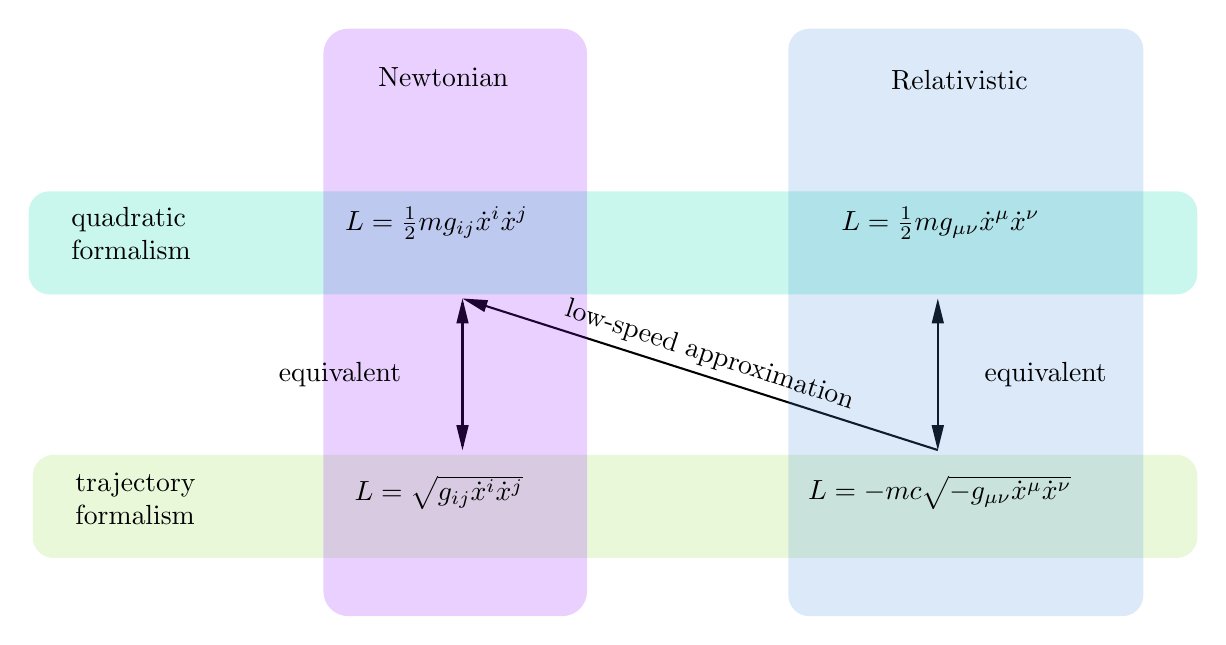
\begin{tikzpicture}[x=0.75pt,y=0.75pt,yscale=-1,xscale=1]
%uncomment if require: \path (0,384); %set diagram left start at 0, and has height of 384

%Straight Lines [id:da7623325543703428] 
\draw    (243,148.67) -- (243,217.67) ;
\draw [shift={(243,219.67)}, rotate = 270] [fill={rgb, 255:red, 0; green, 0; blue, 0 }  ][line width=0.08]  [draw opacity=0] (12,-3) -- (0,0) -- (12,3) -- cycle    ;
\draw [shift={(243,146.67)}, rotate = 90] [fill={rgb, 255:red, 0; green, 0; blue, 0 }  ][line width=0.08]  [draw opacity=0] (12,-3) -- (0,0) -- (12,3) -- cycle    ;
%Straight Lines [id:da2569465613685389] 
\draw    (472,148.67) -- (472,217.67) ;
\draw [shift={(472,219.67)}, rotate = 270] [fill={rgb, 255:red, 0; green, 0; blue, 0 }  ][line width=0.08]  [draw opacity=0] (12,-3) -- (0,0) -- (12,3) -- cycle    ;
\draw [shift={(472,146.67)}, rotate = 90] [fill={rgb, 255:red, 0; green, 0; blue, 0 }  ][line width=0.08]  [draw opacity=0] (12,-3) -- (0,0) -- (12,3) -- cycle    ;
%Rounded Rect [id:dp8999512925345985] 
\draw  [draw opacity=0][fill={rgb, 255:red, 80; green, 227; blue, 194 }  ,fill opacity=0.3 ] (34,104.93) .. controls (34,99.45) and (38.45,95) .. (43.93,95) -- (587.07,95) .. controls (592.55,95) and (597,99.45) .. (597,104.93) -- (597,134.73) .. controls (597,140.22) and (592.55,144.67) .. (587.07,144.67) -- (43.93,144.67) .. controls (38.45,144.67) and (34,140.22) .. (34,134.73) -- cycle ;
%Rounded Rect [id:dp555270186695668] 
\draw  [draw opacity=0][fill={rgb, 255:red, 184; green, 233; blue, 134 }  ,fill opacity=0.3 ] (36,231.93) .. controls (36,226.45) and (40.45,222) .. (45.93,222) -- (587.07,222) .. controls (592.55,222) and (597,226.45) .. (597,231.93) -- (597,261.73) .. controls (597,267.22) and (592.55,271.67) .. (587.07,271.67) -- (45.93,271.67) .. controls (40.45,271.67) and (36,267.22) .. (36,261.73) -- cycle ;
%Straight Lines [id:da6078259469899183] 
\draw    (472,219.67) -- (244.91,147.27) ;
\draw [shift={(243,146.67)}, rotate = 17.68] [fill={rgb, 255:red, 0; green, 0; blue, 0 }  ][line width=0.08]  [draw opacity=0] (12,-3) -- (0,0) -- (12,3) -- cycle    ;
%Rounded Rect [id:dp6948384732062591] 
\draw  [draw opacity=0][fill={rgb, 255:red, 144; green, 19; blue, 254 }  ,fill opacity=0.2 ] (176,28.57) .. controls (176,22) and (181.33,16.67) .. (187.91,16.67) -- (291.09,16.67) .. controls (297.67,16.67) and (303,22) .. (303,28.57) -- (303,287.76) .. controls (303,294.34) and (297.67,299.67) .. (291.09,299.67) -- (187.91,299.67) .. controls (181.33,299.67) and (176,294.34) .. (176,287.76) -- cycle ;
%Rounded Rect [id:dp2732755345951299] 
\draw  [draw opacity=0][fill={rgb, 255:red, 74; green, 144; blue, 226 }  ,fill opacity=0.2 ] (400,26.67) .. controls (400,21.14) and (404.48,16.67) .. (410,16.67) -- (561,16.67) .. controls (566.52,16.67) and (571,21.14) .. (571,26.67) -- (571,289.67) .. controls (571,295.19) and (566.52,299.67) .. (561,299.67) -- (410,299.67) .. controls (404.48,299.67) and (400,295.19) .. (400,289.67) -- cycle ;

% Text Node
\draw (424,100.9) node [anchor=north west][inner sep=0.75pt]    {$L=\frac{1}{2} mg_{\mu \nu }\dot{x}^{\mu }\dot{x}^{\nu }$};
% Text Node
\draw (408,230.4) node [anchor=north west][inner sep=0.75pt]    {$L=-mc\sqrt{-g_{\mu \nu }\dot{x}^{\mu }\dot{x}^{\nu }}$};
% Text Node
\draw (185,100.9) node [anchor=north west][inner sep=0.75pt]    {$L=\frac{1}{2} mg_{ij}\dot{x}^{i}\dot{x}^{j}$};
% Text Node
\draw (189.5,230.4) node [anchor=north west][inner sep=0.75pt]    {$L=\sqrt{g_{ij}\dot{x}^{i}\dot{x}^{j}}$};
% Text Node
\draw (153,176) node [anchor=north west][inner sep=0.75pt]   [align=left] {equivalent};
% Text Node
\draw (493,176) node [anchor=north west][inner sep=0.75pt]   [align=left] {equivalent};
% Text Node
\draw (293.76,144.3) node [anchor=north west][inner sep=0.75pt]  [rotate=-18] [align=left] {low-speed approximation};
% Text Node
\draw (53,101) node [anchor=north west][inner sep=0.75pt]   [align=left] {quadratic\\formalism};
% Text Node
\draw (55,229) node [anchor=north west][inner sep=0.75pt]   [align=left] {trajectory \\formalism};
% Text Node
\draw (201,34) node [anchor=north west][inner sep=0.75pt]   [align=left] {Newtonian};
% Text Node
\draw (448,35) node [anchor=north west][inner sep=0.75pt]   [align=left] {Relativistic};


\end{tikzpicture}
